\documentclass[11pt,a4paper]{article}
\usepackage[margin=2cm,top=1.8cm,bottom=1.8cm]{geometry}
% Préambule commun aux deux documents
\usepackage[T1]{fontenc}
\usepackage[french]{babel}
\usepackage{lmodern}
\usepackage{graphicx,xcolor,booktabs,array,tabularx,longtable}
\usepackage{tikz}
\usetikzlibrary{positioning,arrows.meta,shapes.geometric,calc,fit,backgrounds,decorations.pathreplacing}
\usepackage{fancyhdr,enumitem,microtype}
\usepackage[colorlinks=true,linkcolor=insared,urlcolor=insared,citecolor=insared]{hyperref}
\usepackage{caption}
\usepackage{listings}

\definecolor{insared}{RGB}{200,16,46}
\definecolor{grisfond}{RGB}{247,248,250}
\definecolor{grisligne}{RGB}{216,220,226}
\definecolor{gristexte}{RGB}{91,97,107}
\definecolor{vertok}{RGB}{26,127,75}
\definecolor{orangepartiel}{RGB}{178,106,5}
\definecolor{rougeko}{RGB}{198,40,40}

\captionsetup{font=small,labelfont={bf,color=insared}}
\setlist[itemize]{leftmargin=1.2em,itemsep=1pt,topsep=2pt,parsep=0pt}
\setlist[enumerate]{leftmargin=1.4em,itemsep=1pt,topsep=2pt,parsep=0pt}

\lstset{
  basicstyle=\ttfamily\scriptsize,
  backgroundcolor=\color{grisfond},
  frame=single, rulecolor=\color{grisligne},
  breaklines=true, showstringspaces=false,
  keywordstyle=\color{insared}\bfseries,
  commentstyle=\color{gristexte}\itshape,
  numberstyle=\tiny\color{gristexte},
  xleftmargin=4pt, framexleftmargin=4pt, aboveskip=6pt, belowskip=6pt,
  literate={é}{{\'e}}1 {è}{{\`e}}1 {à}{{\`a}}1 {ç}{{\c c}}1 {ê}{{\^e}}1 {û}{{\^u}}1 {î}{{\^i}}1 {ô}{{\^o}}1 {É}{{\'E}}1 {—}{{---}}1 {’}{{'}}1 {«}{{<<}}1 {»}{{>>}}1 {·}{{\textperiodcentered}}1
}

% Marqueurs de conformité
\newcommand{\ok}{\textcolor{vertok}{\textbf{Conforme}}}
\newcommand{\partiel}{\textcolor{orangepartiel}{\textbf{Partiel}}}
\newcommand{\absent}{\textcolor{rougeko}{\textbf{Absent}}}
\newcommand{\plus}{\textcolor{insared}{\textbf{Au-delà}}}

% Les paragraphes techniques enchaînent de longues suites en \texttt{} que TeX
% ne peut pas couper : sans marge de man\oe{}uvre, elles débordent dans la marge.
% \emergencystretch autorise un dernier passage plus souple sur ces lignes-là.
\emergencystretch=2em
\hbadness=4000        % ne pas signaler les lignes simplement peu denses


\pagestyle{fancy}\fancyhf{}
\renewcommand{\headrulewidth}{0.4pt}
\fancyhead[L]{\small\textcolor{gristexte}{InsaCloud --- Projet 3}}
\fancyhead[R]{\small\textcolor{gristexte}{Outils de déploiement de plateformes}}
\fancyfoot[C]{\small\thepage\ / \pageref{LastPage}}
\usepackage{lastpage}

\setlength{\parskip}{3pt}
\setlength{\parindent}{0pt}

\begin{document}

%================================================================ TITRE
\begin{center}
{\LARGE\bfseries InsaCloud}\\[2pt]
{\large Location de conteneurs Linux à la demande, avec accès SSH et haute disponibilité}\\[6pt]
{\small Mohamed Aziz BAOUEB \quad\textbullet\quad STI 4A FISE \quad\textbullet\quad Projet 3\\
Outils de déploiement de plateformes --- Dr. Nadia FETTAH \quad\textbullet\quad 2026/2027}\\[2pt]
{\small\textcolor{gristexte}{Code source : \url{https://github.com/aziz3r/insacloud}}}
\end{center}
\vspace{-4pt}
\rule{\linewidth}{0.8pt}

%================================================================ 1
\section{Introduction}

\textbf{Objectif du projet.} InsaCloud est une application web Flask qui permet à un visiteur de créer
un compte, puis de \emph{louer} depuis un tableau de bord une machine (conteneur Docker) de la
distribution et pour la durée de son choix. Un accès SSH lui est remis au moment de la location,
et le service reste disponible même en cas de crash de l'instance ou perte d'accès.

\textbf{Portée du document.} Ce rapport décrit l'architecture retenue, les fonctionnalités livrées et
vérifiées, les difficultés rencontrées et les pistes d'évolution. Le projet, prévu pour un groupe
de quatre à cinq personnes, a été réalisé seul : les quatre catégories de tâches de l'énoncé
(API web, partie Ansible, base de données, déploiement des machines) ont donc toutes été menées
par le même auteur. Un \emph{dossier technique} complémentaire détaille la synthèse de cours et
l'analyse de conformité point par point.

\textbf{Périmètre fonctionnel.} Trois distributions (Ubuntu~22.04, Debian~12, Alpine~3.20), deux modes
d'accès (terminal ou bureau graphique), durée de 1 à 120~minutes prolongeable, quota de trois machines
par utilisateur, destruction automatique à l'expiration.

%================================================================ 2
\section{Aperçu de l'architecture}

\begin{figure}[h]\centering
\begin{tikzpicture}[font=\scriptsize,node distance=6mm,
  boite/.style={draw=grisligne,fill=grisfond,rounded corners=2pt,inner sep=4pt,align=center},
  titre/.style={font=\scriptsize\bfseries}]
\node[boite,minimum width=2cm,minimum height=1.1cm] (nav) {Navigateur\\[-1pt]\textcolor{gristexte}{utilisateur}};
\node[draw=grisligne,rounded corners=3pt,inner sep=5pt,right=14mm of nav,minimum width=3.6cm,minimum height=3.4cm] (ctrl) {};
\node[titre,color=insared] at ([yshift=-5mm]ctrl.north) {controller --- 192.168.56.10};
\node[boite,minimum width=3cm] (n1) at ([yshift=-11mm]ctrl.north) {nginx \textperiodcentered{} TLS 1.3};
\node[boite,minimum width=3cm,below=1.5mm of n1] (n2) {Gunicorn \textperiodcentered{} Flask};
\node[boite,minimum width=3cm,below=1.5mm of n2] (n3) {Faucheur \textperiodcentered{} Watchdog};
\node[boite,minimum width=3cm,below=1.5mm of n3] (n4) {SQLite \textperiodcentered{} Vault};
\node[draw=grisligne,rounded corners=3pt,inner sep=5pt,right=16mm of ctrl,yshift=10mm,minimum width=3.7cm,minimum height=1.35cm] (w1) {};
\node[titre] at ([yshift=-4mm]w1.north) {worker1 --- .56.11};
\node[boite,minimum width=3.1cm,font=\tiny] at ([yshift=-11mm]w1.north) {dockerd \textperiodcentered\ live-restore\\conteneurs insacloud\_*};
\node[draw=grisligne,rounded corners=3pt,inner sep=5pt,below=6mm of w1,minimum width=3.7cm,minimum height=1.35cm] (w2) {};
\node[titre] at ([yshift=-4mm]w2.north) {worker2 --- .56.12};
\node[boite,minimum width=3.1cm,font=\tiny] at ([yshift=-11mm]w2.north) {dockerd \textperiodcentered\ live-restore\\conteneurs insacloud\_*};
\draw[-{Stealth},thick] (nav) -- node[above,font=\tiny]{HTTPS} (ctrl);
\draw[-{Stealth}] (ctrl.east) -- node[above,font=\tiny,pos=.55]{docker -H ssh://} (w1.west);
\draw[-{Stealth}] (ctrl.east) -- (w2.west);
\draw[-{Stealth},dashed] (nav.south) |- ([yshift=-8mm]$(w2.south)!0.5!(w2.south)$) node[below,font=\tiny,pos=.75]{SSH \textperiodcentered\ terminal web \textperiodcentered\ bureau (ports 8000--9000)} -| (w2.south);
\end{tikzpicture}
\caption{Architecture déployée : un contrôleur et deux \emph{workers}, provisionnés par Vagrant et Ansible.}
\end{figure}

\textbf{Séparation contrôleur / workers.} Le serveur web ne doit pas être le point de défaillance
unique de l'exécution. Le contrôleur héberge donc uniquement le site, la base et les démons de
supervision ; il n'exécute \emph{aucun} conteneur loué et ne possède même pas de démon Docker, mais
seulement le client. Les machines louées vivent sur des \emph{workers} dédiés.

\textbf{Pilotage des workers par SSH.} Plutôt que d'exposer l'API Docker sur le réseau (risque
d'élévation de privilèges équivalente à un accès \texttt{root}), le contrôleur utilise le transport
natif du client Docker : \texttt{docker -H ssh://insacloud@worker1}. L'authentification se fait par
clé dédiée, générée par Ansible et déposée sur les workers, pour un compte sans mot de passe.

\textbf{Placement des machines.} À chaque location, l'application interroge la base pour compter les
machines actives par n\oe{}ud et choisit le moins chargé --- un ordonnanceur simple, déterministe et
lisible, suffisant pour un parc de cette taille.

\textbf{Haute disponibilité à deux niveaux.} Dans chaque machine, \texttt{supervisord} s'exécute en
PID~1 et relance individuellement les services (sshd, terminal web, serveur d'affichage, bureau) ;
si supervisord meurt, Docker relance le conteneur grâce à \texttt{-{}-restart=always}. Le démon Docker
des workers est configuré en \texttt{live-restore} : une mise à jour de Docker n'interrompt pas les
machines en cours.

\textbf{Nettoyage par un démon dédié (\og{} le Faucheur \fg{}).} Un service séparé lit la base toutes les dix
secondes et détruit les machines expirées. Il réalise aussi une \emph{réconciliation} : un conteneur
inconnu de la base est supprimé, une machine sans conteneur est marquée arrêtée, et un worker
injoignable est ignoré plutôt qu'interprété comme une disparition.

\textbf{Auto-réparation du service (watchdog).} Un \emph{timer} systemd vérifie chaque minute nginx,
la réponse HTTPS du site et le Faucheur, redémarre ce qui est tombé et journalise les workers
injoignables.

\textbf{Infrastructure comme code.} Un \texttt{Vagrantfile} décrit les trois machines virtuelles ;
un playbook Ansible de huit rôles les configure intégralement. Le playbook est idempotent :
un second passage renvoie \texttt{changed=0} sur les trois n\oe{}uds.

\textbf{Gestion des secrets.} Les clés sensibles (session Flask, chiffrement des mots de passe) sont
stockées chiffrées dans un fichier Ansible Vault, et déposées sur le serveur dans un fichier en
permissions \texttt{0600} lu par systemd --- jamais dans une unité ni dans les journaux.

%================================================================ 3
\section{Fonctionnalités}

\subsection*{Comptes et tableau de bord}
Inscription et connexion (mots de passe hachés PBKDF2 salé), verrouillage après cinq échecs,
redirection vers un tableau de bord qui liste les machines, leur état Docker réel, le temps restant
et les actions disponibles.

\begin{figure}[h]\centering
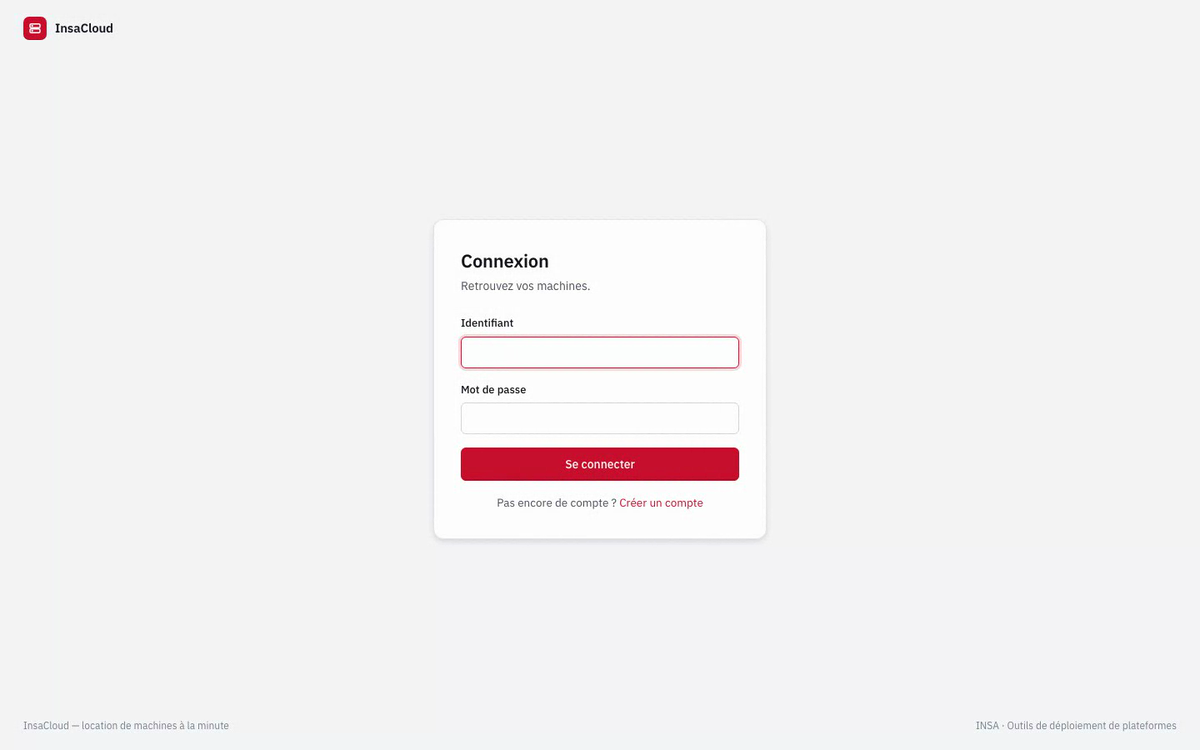
\includegraphics[width=0.485\linewidth]{../docs/01-connexion.png}\hfill
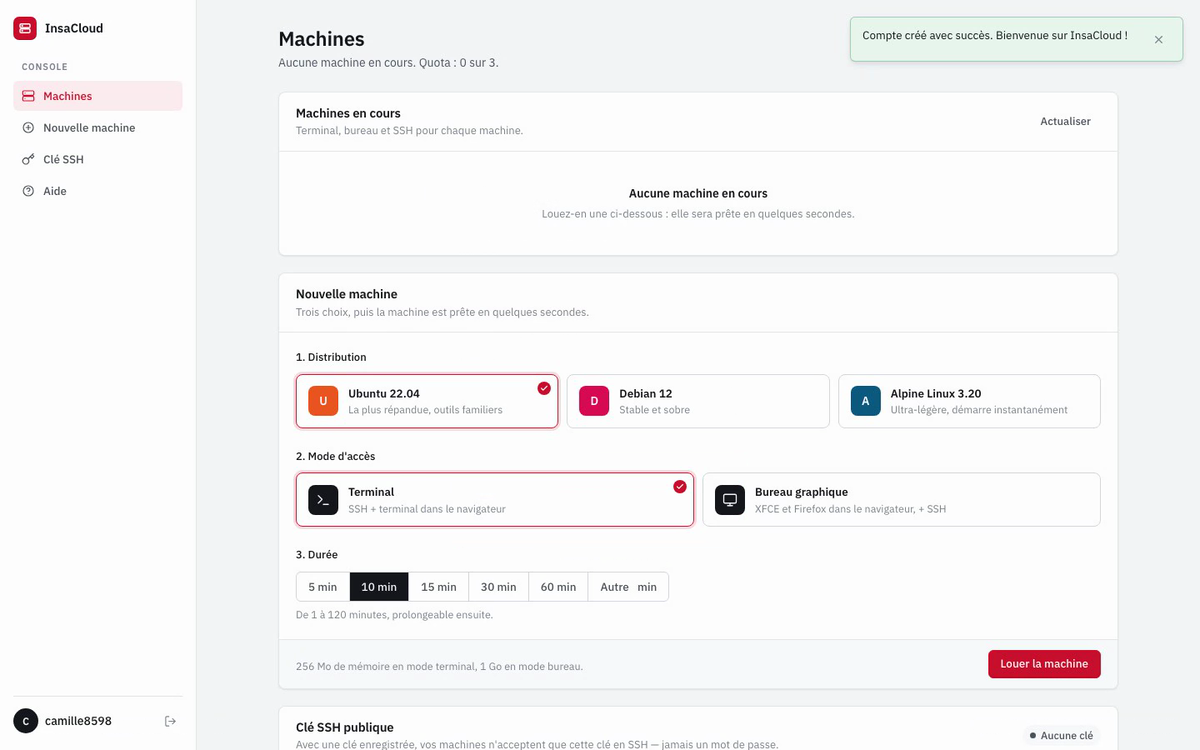
\includegraphics[width=0.485\linewidth]{../docs/03-tableau-de-bord.png}
\caption{Connexion (gauche) et tableau de bord avec le formulaire de location en trois choix (droite).}
\end{figure}

\subsection*{Location : distribution, mode et durée}
Trois distributions et deux modes d'accès, soit six images construites à partir de trois
\texttt{Dockerfile} (la variante bureau s'active par \texttt{-{}-build-arg DESKTOP=1}). La commande
effectivement exécutée est :

\begin{lstlisting}[language=bash]
docker run -d --restart=always -p <p1>:22 -p <p2>:7681 [-p <p3>:6080] \
  --name insacloud_<user>_<id> -e ROOT_PASSWORD=<aleatoire> [-e SSH_PUBKEY=...] \
  --cap-drop ALL --cap-add CHOWN ... --security-opt no-new-privileges:true \
  --pids-limit 512 --cpus 1 --memory 256m|1g  insacloud_<distro>[_desktop]:latest
\end{lstlisting}

\subsection*{Accès SSH remis à la location}
La commande exacte (\texttt{ssh root@<hôte> -p <port>}) est affichée sur la carte de la machine.
Le mot de passe \texttt{root} est tiré au sort (16 caractères), affiché \emph{une seule fois},
puis conservé chiffré ; il peut être régénéré à chaud. L'utilisateur peut enregistrer sa clé
publique SSH : ses machines n'acceptent alors plus que cette clé.

\begin{figure}[h]\centering
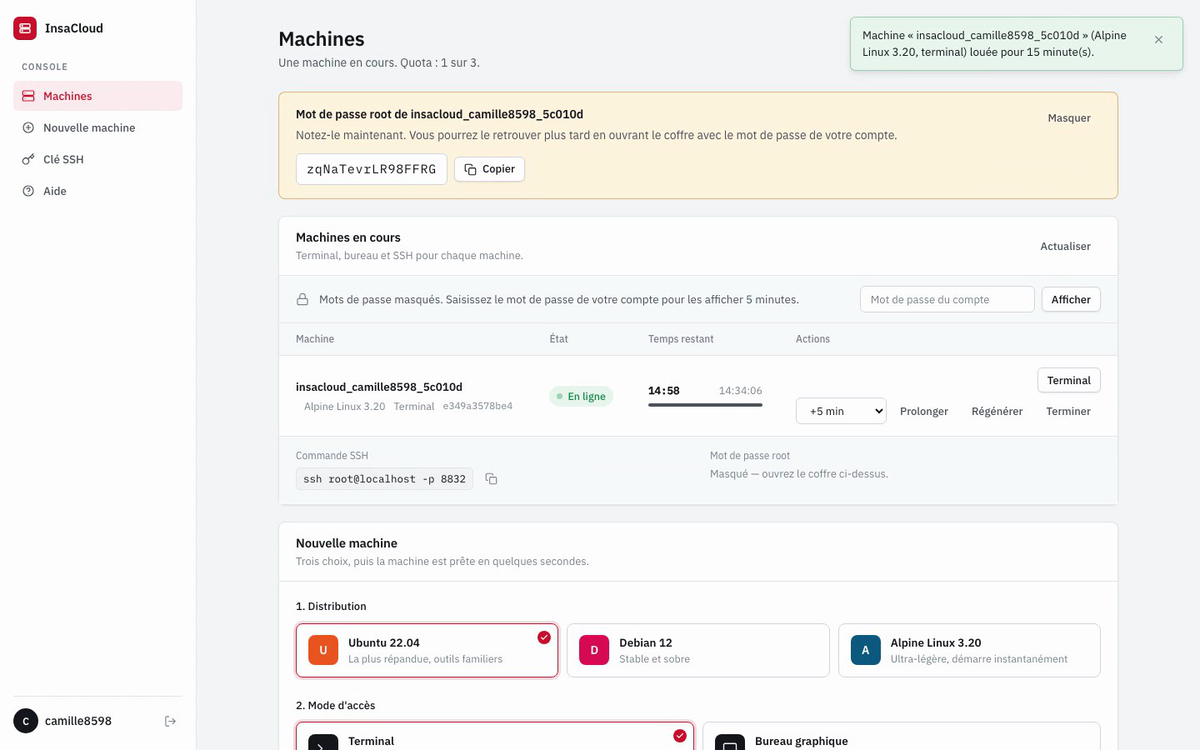
\includegraphics[width=0.485\linewidth]{../docs/05-mot-de-passe-unique.png}\hfill
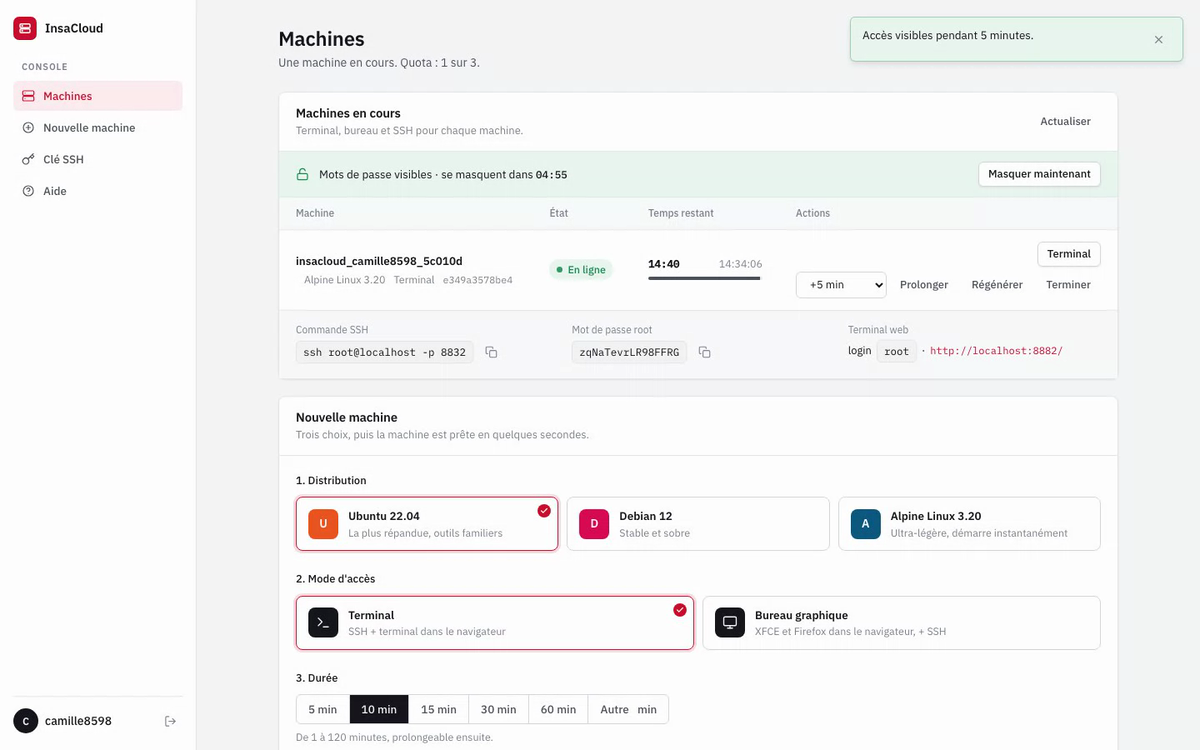
\includegraphics[width=0.485\linewidth]{../docs/06-coffre-ouvert.png}
\caption{Mot de passe affiché une seule fois (gauche) ; coffre rouvert après re-authentification (droite).}
\end{figure}

\subsection*{Accès sans client : terminal et bureau dans le navigateur}
Chaque machine expose un terminal web (\texttt{ttyd}) avec une invite de connexion classique, et,
en mode bureau, un environnement XFCE complet avec Firefox diffusé par noVNC.

\begin{figure}[h]\centering

\includegraphics[width=0.485\linewidth]{../docs/07-terminal-web.png}\hfill
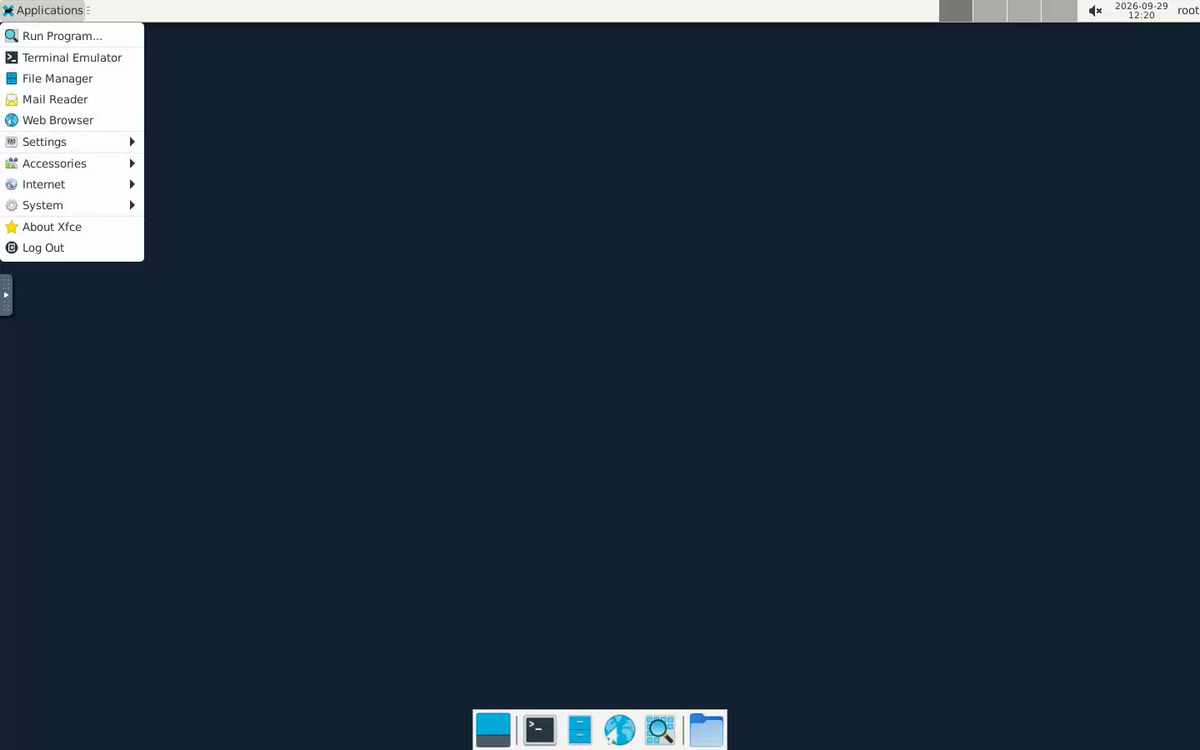
\includegraphics[width=0.485\linewidth]{../docs/09-bureau-applications.png}
\caption{Terminal web (gauche) et bureau XFCE dans le navigateur (droite).}
\end{figure}

\subsection*{Haute disponibilité et expiration}
Vérifications réalisées sur banc de test à trois n\oe{}uds : un worker entièrement redémarré retrouve
ses machines \emph{et} les fichiers créés à l'intérieur ; un service arrêté de force est relancé par
le watchdog en moins d'une minute ; une machine expirée est détruite par le Faucheur dans les
secondes qui suivent (mesuré : expiration 15:13:48, destruction 15:13:52).

\subsection*{Automatisation complète}
\texttt{vagrant up} crée les trois VM ; \texttt{ansible-playbook site.yml -{}-ask-vault-pass} installe
pare-feu, Docker, certificats, images, nginx et application. Résultats mesurés : premier passage
\texttt{ok=72 / changed=35 / failed=0} sur le contrôleur et \texttt{ok=57 / changed=21} sur chaque
worker ; second passage \texttt{changed=0} sur les trois n\oe{}uds.

\subsection*{Sécurité}
Jetons CSRF sur tous les formulaires, politique de mot de passe, cookies \texttt{Secure} /
\texttt{HttpOnly} / \texttt{SameSite=Strict}, en-têtes de sécurité avec une CSP
\texttt{default-src 'self'} (aucun CDN, aucun script en ligne), HTTPS de bout en bout,
pare-feu UFW différencié par groupe, conteneurs à capacités minimales.

%================================================================ 4
\section{Difficultés}

\textbf{La politique \texttt{-{}-restart=always} ne se déclenche pas après un \texttt{docker kill}.}
Docker distingue volontairement un arrêt manuel d'un crash. La démonstration de résilience passe
donc par la mort du processus \emph{à l'intérieur} du conteneur (\texttt{kill -TERM 1}), ce qui
relance bien le conteneur (\texttt{RestartCount: 1}).

\textbf{Terminal web inutilisable derrière une authentification HTTP.} Protégé par
\texttt{Basic Auth}, le terminal affichait une page blanche dans plusieurs navigateurs. Le
remplacement par \texttt{/bin/login} dans le terminal a rendu l'expérience familière et plus sûre
(PAM, temporisation entre échecs, expiration de l'invite).

\textbf{Contraintes des images de distribution.} Ubuntu ne fournit Firefox qu'en paquet Snap,
inutilisable en conteneur : il a fallu passer par le dépôt APT officiel de Mozilla. \texttt{ttyd}
n'est pas empaqueté dans Debian~12 : binaire statique officiel. Enfin, le nom du binaire de mot de
passe VNC diffère selon la distribution, d'où une détection à l'exécution.

\textbf{Un mot de passe VNC est limité à huit caractères} par le protocole : il a fallu exposer un
mot de passe de bureau distinct et chiffrer le transport.

\textbf{Docker dans Docker pour tester le cluster.} Le banc de test (trois conteneurs systemd
simulant les VM) échouait au \texttt{docker build} : le pilote overlay ne peut pas se superposer
à lui-même. La solution a été de monter \texttt{/var/lib/docker} et \texttt{/var/lib/containerd}
sur des volumes Docker dédiés.

\textbf{Deux tâches Ansible en conflit sur le même répertoire.} Le rôle \texttt{controller\_key}
créait \texttt{.ssh} en \texttt{0700} et le rôle \texttt{webapp} le remettait en \texttt{0755} :
chaque exécution affichait un \texttt{changed}. Le retrait du doublon a rendu le playbook
parfaitement idempotent.

\textbf{PEP 668.} Depuis Ubuntu~23.04, \texttt{pip install} est interdit hors environnement virtuel,
ce qui impose de créer un \emph{virtualenv} dans le rôle Ansible.

%================================================================ 5
\section{Orientations futures}

\textbf{Déjà comblé depuis la première version.} La relecture du cours avait révélé huit écarts, tous
traités depuis : un fichier \texttt{docker-compose.yml} déclare la construction des images et une
machine de démonstration ; chaque conteneur reçoit désormais une \emph{réservation} mémoire en plus
de sa limite ; la construction des images est encadrée par \texttt{block}/\texttt{rescue}/\texttt{always} ;
le \texttt{Vagrantfile} enchaîne lui-même le \emph{provisioner} Ansible ; le \emph{watchdog} relève
la consommation CPU et mémoire de chaque machine (\texttt{docker stats}) ; les huit rôles déclarent
leurs dépendances dans \texttt{meta/main.yml} ; un inventaire dynamique interroge Vagrant ; enfin une
chaîne d'intégration continue exécute à chaque envoi huit contrôles --- lint, 67 tests, SAST, SCA,
recherche de secrets, DAST et scan de l'image Docker.

\textbf{Court terme.} Certificat reconnu (Let's Encrypt) en remplacement du certificat auto-signé,
seule alerte que le scan dynamique signale encore ; quotas de ressources par utilisateur et non plus
seulement par machine ; notification (courriel ou webhook) lorsqu'un worker devient injoignable.

\textbf{Moyen terme.} Authentification à deux facteurs ; journalisation centralisée des accès aux
machines louées ; archivage du travail de l'utilisateur avant destruction, pour que l'expiration
ne soit plus une perte sèche.

\textbf{Long terme.} Passage à un orchestrateur (Docker Swarm ou Kubernetes) si le parc dépasse la
dizaine de n\oe{}uds : la planification, la santé des n\oe{}uds et le redémarrage des conteneurs
seraient alors délégués à l'orchestrateur, et le Faucheur se réduirait à une politique d'expiration.

\end{document}
